%set document class:
\documentclass[11pt,letterpaper]{article}

%configure page margins with geometry package:
\usepackage[left=1.in,right=1.in,footskip=0.5in,bottom=0.5in,top=0.5in,includefoot]{geometry}

%set language (load hyphenation patterns):
\usepackage[english]{babel}

%fonts and input encoding packages:
\usepackage[T1]{fontenc}
\usepackage{lmodern}
\usepackage[utf8]{inputenc}
\usepackage{indentfirst}

%graphics/figures packages:
\usepackage{graphicx}
\usepackage[usenames,dvipsnames]{color}
\usepackage{epstopdf}
\usepackage[labelfont=bf,hypcap=true]{caption}
\usepackage{subcaption}

%load additional (math) fonts:
\usepackage{amsmath}
\usepackage{amsfonts}
\usepackage{amssymb}
\usepackage{bm}
\usepackage{braket}
\usepackage{algorithm}
\usepackage[noend]{algpseudocode}
\makeatletter
\def\BState{\State\hskip-\ALG@thistlm}
\makeatother

%improve spacing between words and letters:
\usepackage{microtype}

%configure cross-references and links:
\usepackage{url}
%(set colorlinks=false to remove colored links)
\usepackage[hyperfootnotes=false,colorlinks=true,citecolor=Blue,
            urlcolor=Blue,linkcolor=Blue,breaklinks=true]{hyperref}

\usepackage{multicol}

%define some additional commands for convenience:
\title{KCores}
%tensor/matrix:
\newcommand{\ten}[1]{\mathsf{#1}}
%vector with bold font:
\renewcommand{\vec}[1]{\mathbf{#1}}
%bold symbol (e.g. for greek letters):
\newcommand{\bs}[1]{\boldsymbol{#1}}
%differential:
\newcommand{\dd}{\,\mathrm{d}}
%partial differential:
\newcommand{\pd}{\partial}
%complex i:
\newcommand{\ii}{\mathrm{i}}


%all content goes between \begin{document} and \end{document}:
\begin{document}

%set title, author, and date:

%\title{\textsc{\large{K-Core Paper}}}  %\\ is for new line
%\author{authors}
%\date{\today}
%make title:
\maketitle


\section*{Simplified K-Core Model}
\begin{equation}\label{eq:kcore}
\dot{V_j} = -\frac{1}{\tau _v} V_j + \Delta V(C_j) \sum_i r(V_i)
\end{equation}
\begin{equation}\label{eq:kcore2}
\dot{C_j} = -\frac{1}{\tau _c} C_j + \Delta C \sum_i r(V_i)
\end{equation}
\begin{equation}\label{eq:k_of_kcore}
V_j = \tau _v \Delta V_{min} K r_{max} \Rightarrow K = \frac{V^*}{\tau _v \Delta V_{min} r_{max}}
\end{equation}


\section*{Step Function, Mean Field}
Modeling the firing rate of neurons with a step function in the mean field limit, we get:
%TODO: CHECK THESE EQUATIONS AGAIN
\begin{equation}\label{eq:step_mean_field}
\dot{V} = -\frac{V}{\tau _v} + n\Delta V \theta (C^* - C)[r_1\theta (V - V^*) + r_0]
\end{equation}
\begin{equation}
\dot{C} = -\frac{C}{\tau _c} + n\Delta C [r_1 \theta (V - V^*) + r_0]
\end{equation}

The dependence of firing rate (P) on voltage (V), and voltage increment ($\Delta V$) on Calcium concentration (Ca) are taken to be step functions (Figure~\ref{fig:step_function}). $\tau _v$ and $tau _c$ are time constants, $r_0$ is minimum firing rate, and n is the total number of neurons in the network.

\begin{figure}[!h]
  \centering
  	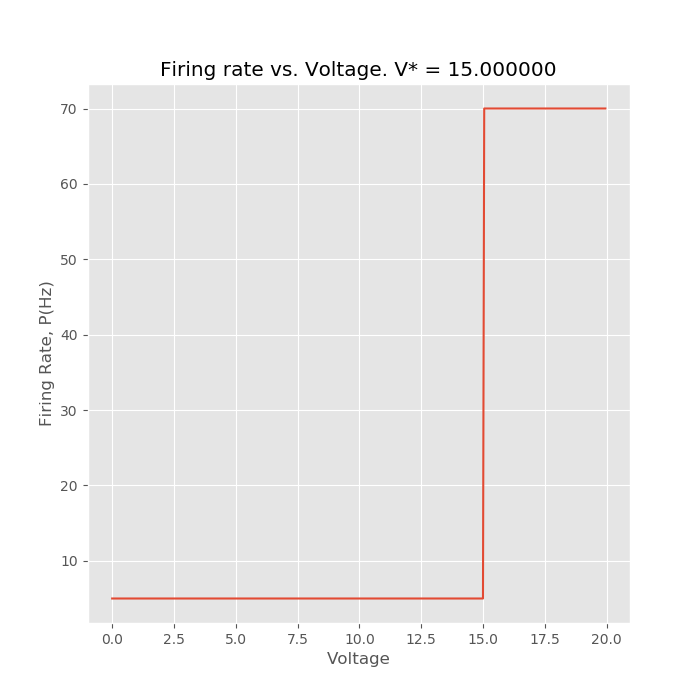
\includegraphics[width=70mm]{firing_rate.png}
    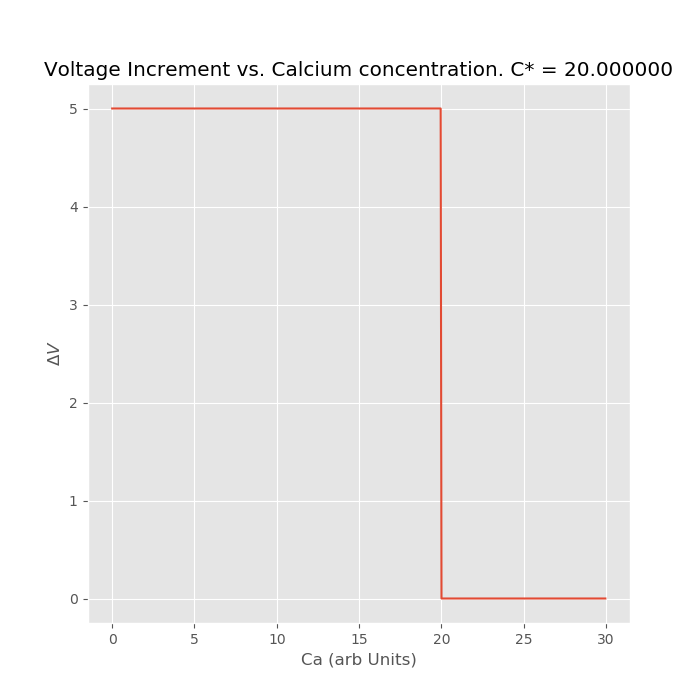
\includegraphics[width=70mm]{delV.png}
  \caption{Left: Neuron firing rate as a function of voltage. Right: Voltage increment dependence on calcium concentration for C* = 20. Above C*, $\Delta V = 0$}
  \label{fig:step_function}
\end{figure}

\subsection*{Case I: $V < V^*, C < C^*$}
For fixed points, we take $\dot{V} = \dot{C} = 0$. $r_0$ is taken to be the low firing rate, while $r_0 + r_1$ is taken to be the maximum firing rate (70 Hz). This results in the following equations for V and C:

\begin{equation}
V = n\tau _v \Delta V r_0
\end{equation}
\begin{equation}
C = n\tau _c \Delta C r_0
\end{equation}

This fixed point is defined as a low voltage fixed point (Figure~\ref{fig:step_function_plots}).

\subsection*{Case II: $V < V^*, C > C^*$}
$\Delta V$ goes to 0 so:
\begin{equation}
V = 0
\end{equation}
\begin{equation}
C = n\tau _c \Delta C r_0
\end{equation}
%TODO: CHECK LAST 3 EQUATIONS ON THIS PAGE
\subsection*{Case III: $V > V^*, C > C^*$}
$\Delta V$ goes to 0 so:
\begin{equation}
V = 0
\end{equation}
\begin{equation}
C = n\tau _c \Delta C(r_1 + r_0)
\end{equation}

\subsection*{Case IV: $V > V^*, C < C^*$}
\begin{equation}
V = n\tau_v \Delta V (r_1 + r_0)
\end{equation}
\begin{equation}
C = n\tau_c \Delta C (r_1 + r_0)
\end{equation}
The phase diagram has a high voltage fixed point (Figure~\ref{fig:step_function_plots}).

\begin{figure}[h!]
  \centering
  	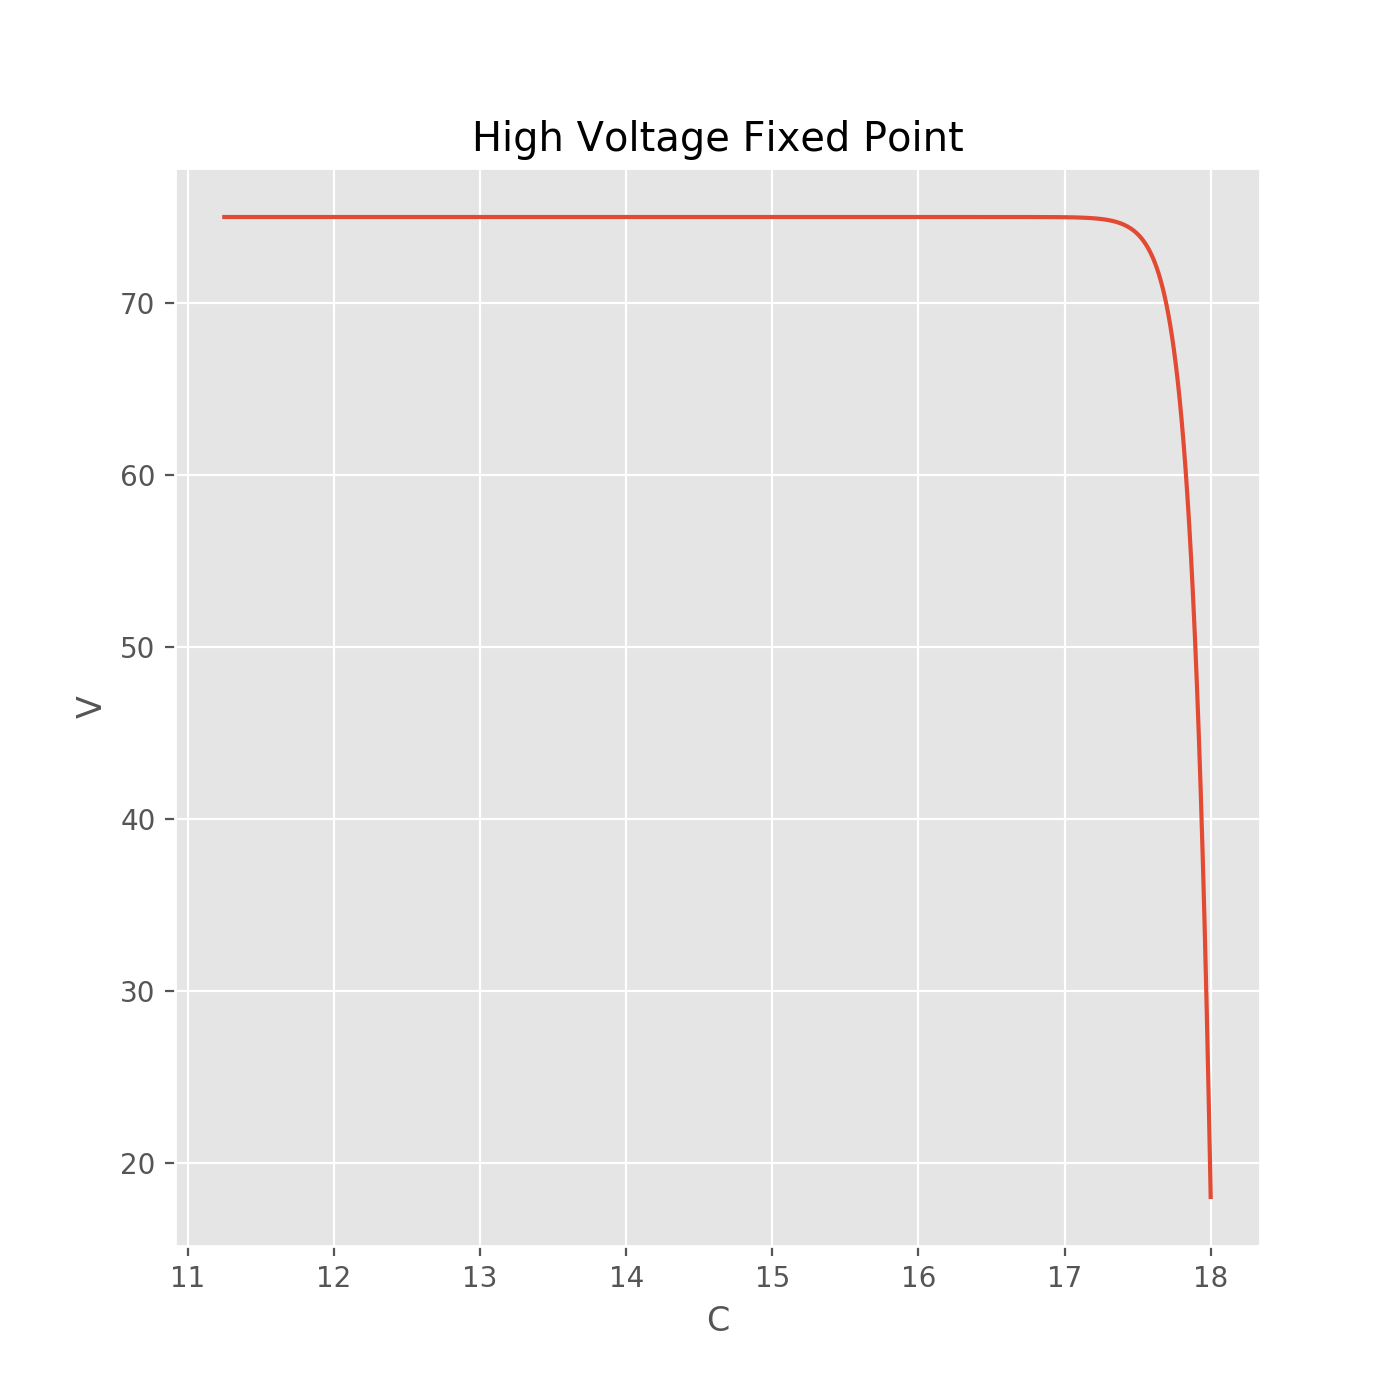
\includegraphics[width=70mm]{step_high.png}
    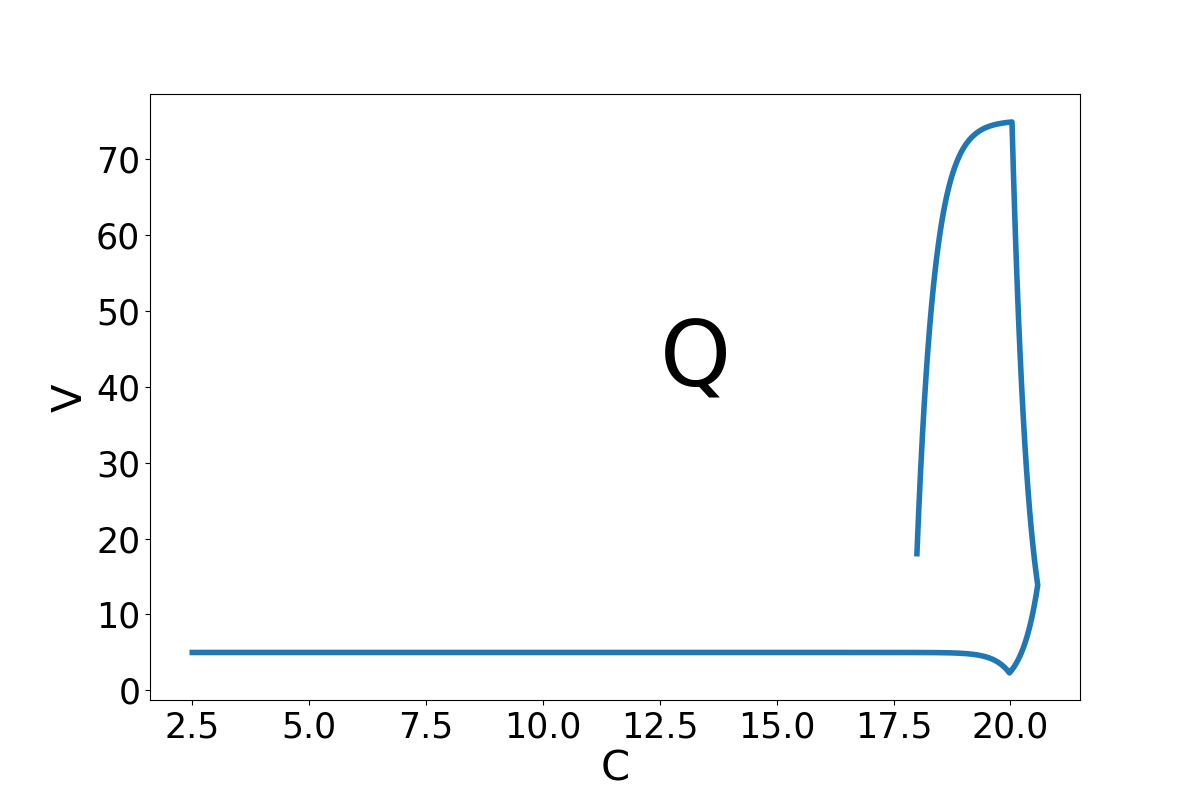
\includegraphics[width=70mm]{step_low.png}\\
    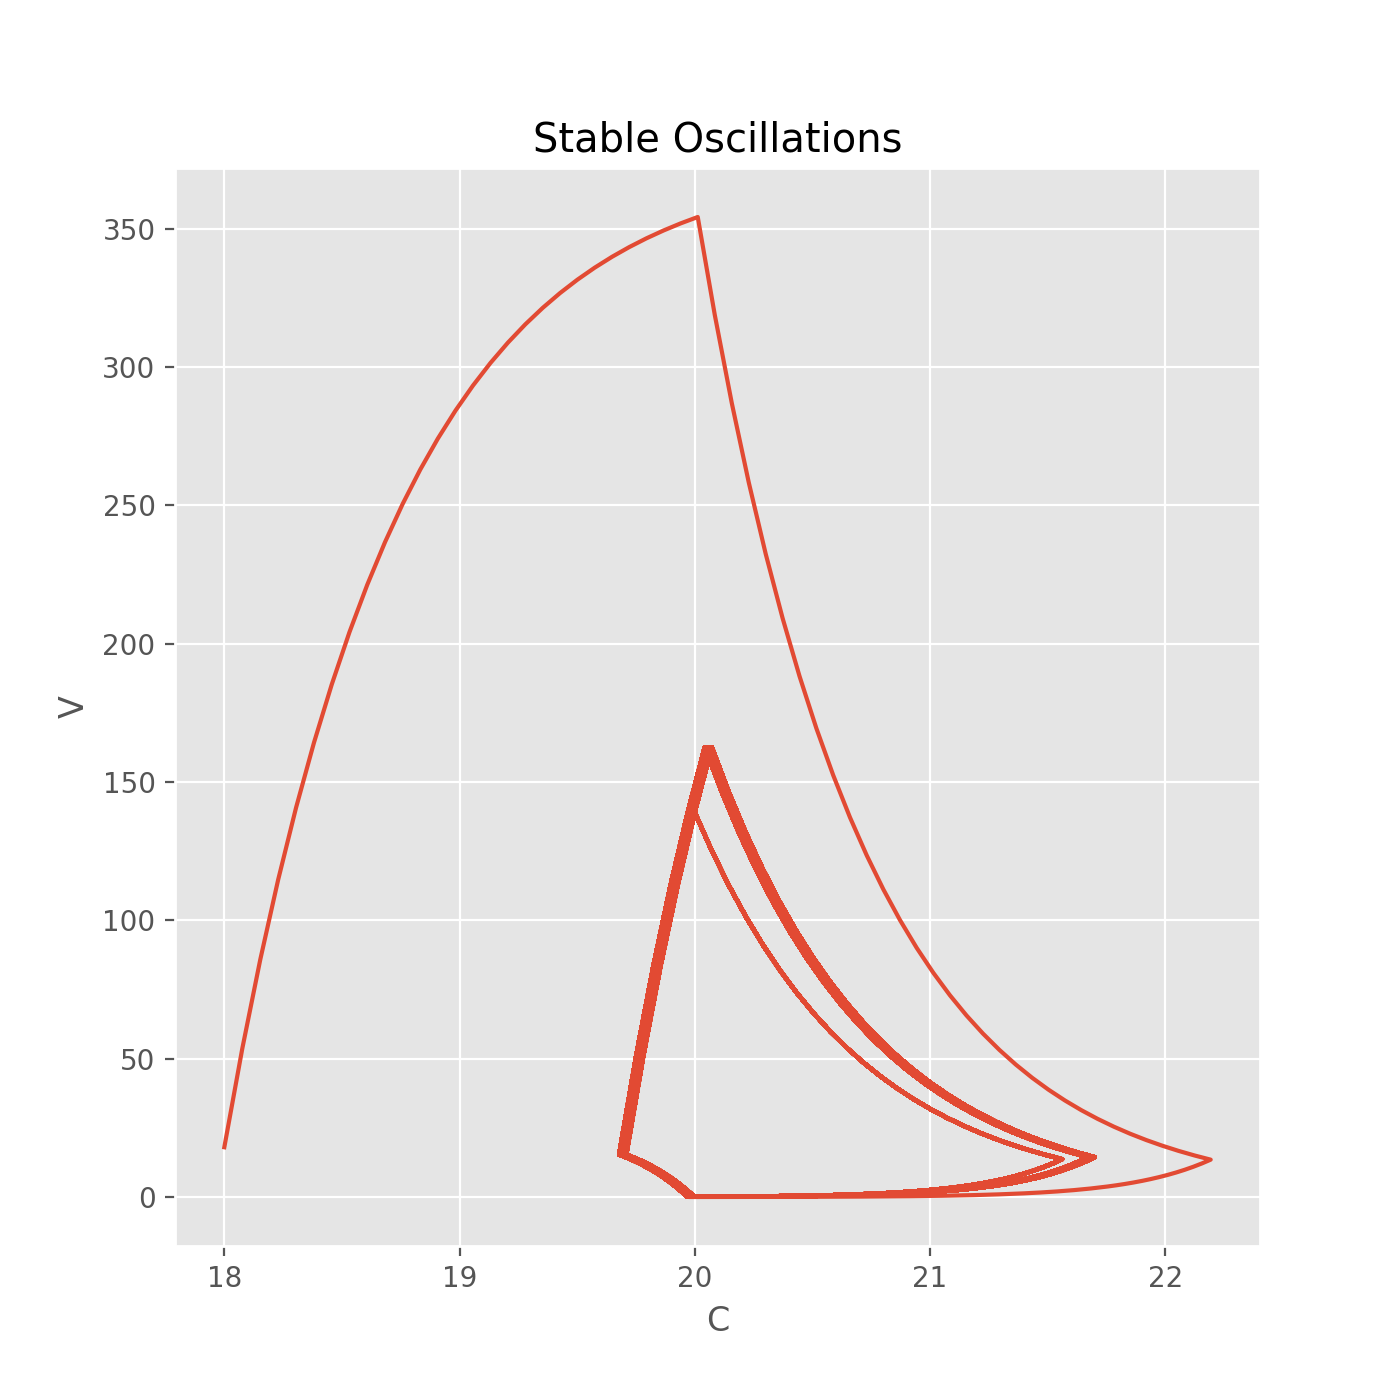
\includegraphics[width = 70mm]{step_SO.png}
  \caption{Top Left: High Voltage Fixed point. Top Right: Low Voltage Fixed Point. Bottom: Stable Oscillation.}
  \label{fig:step_function_plots}
\end{figure}

\subsection*{Network Connectivity Analysis}
Phase diagrams for the network are plotted as a function of network size according to parameter $\Delta V$ and $\Delta C$ (Figure~\ref{fig:step_function_phase_diagrams}).

\begin{figure}[h!]
  \centering
  	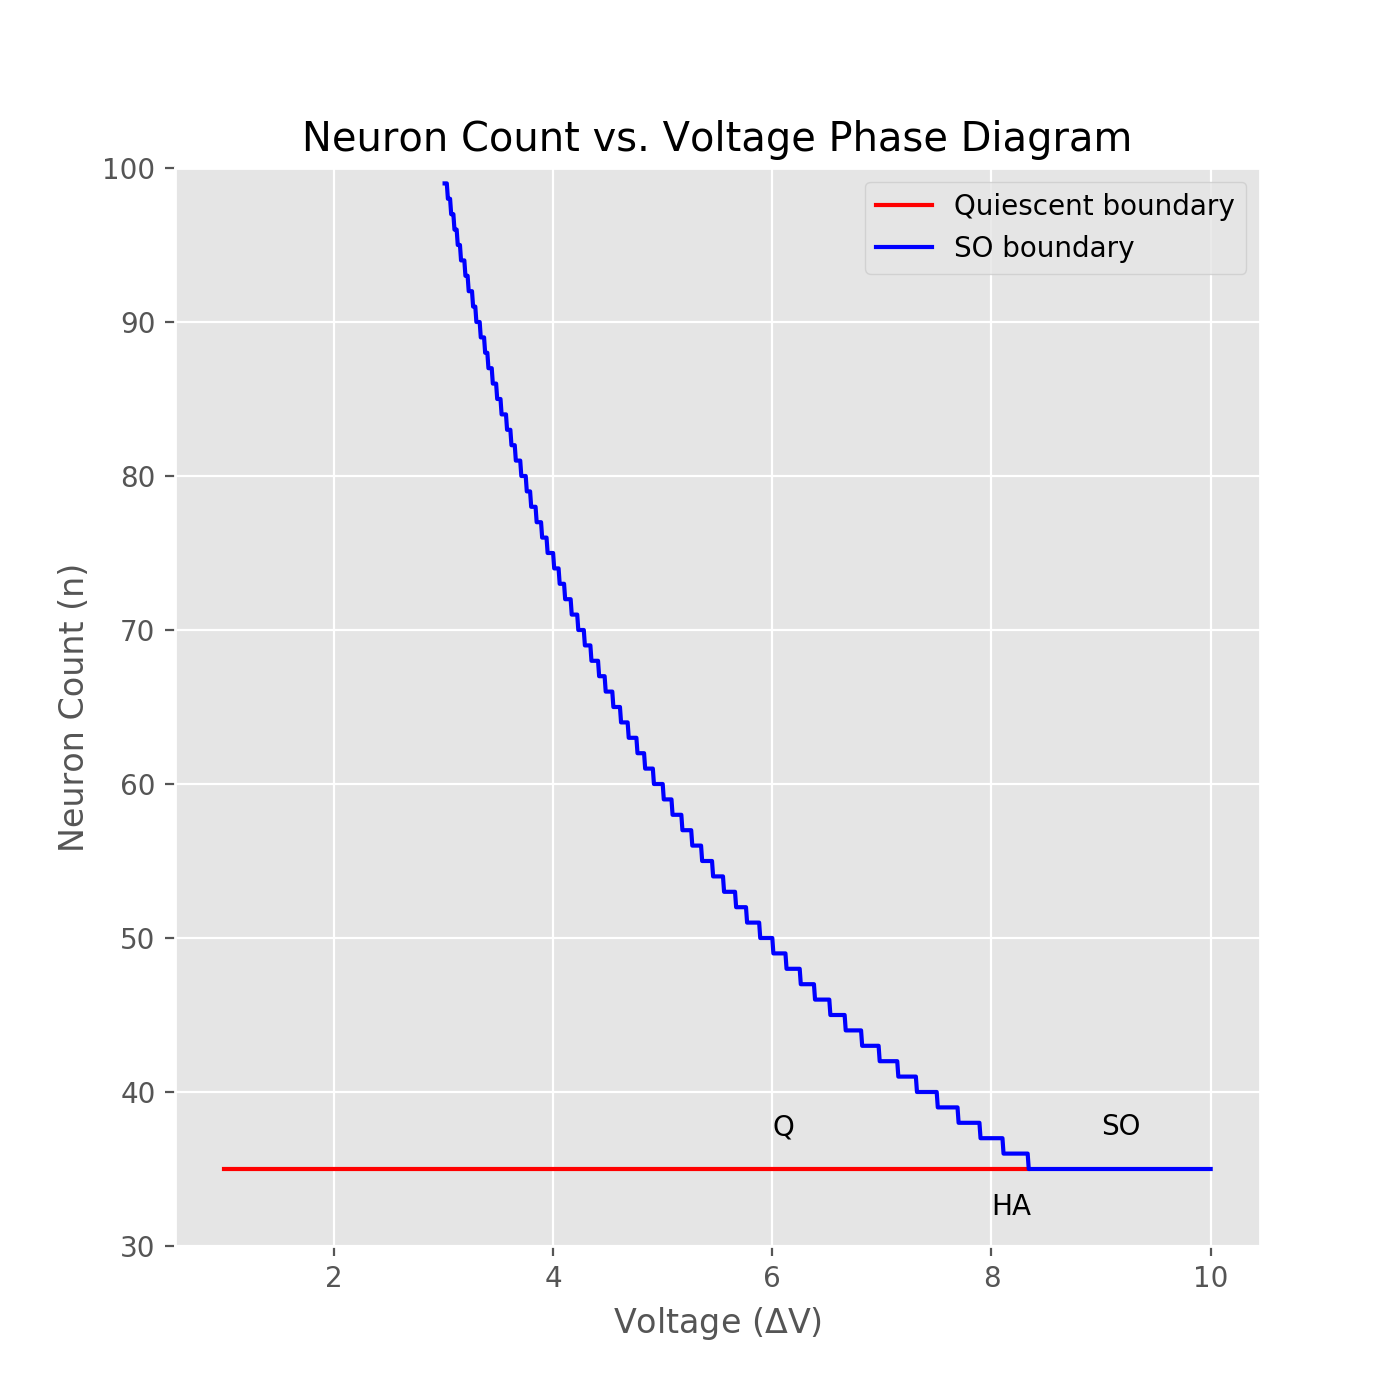
\includegraphics[width=70mm]{step_nV_phase.png}
    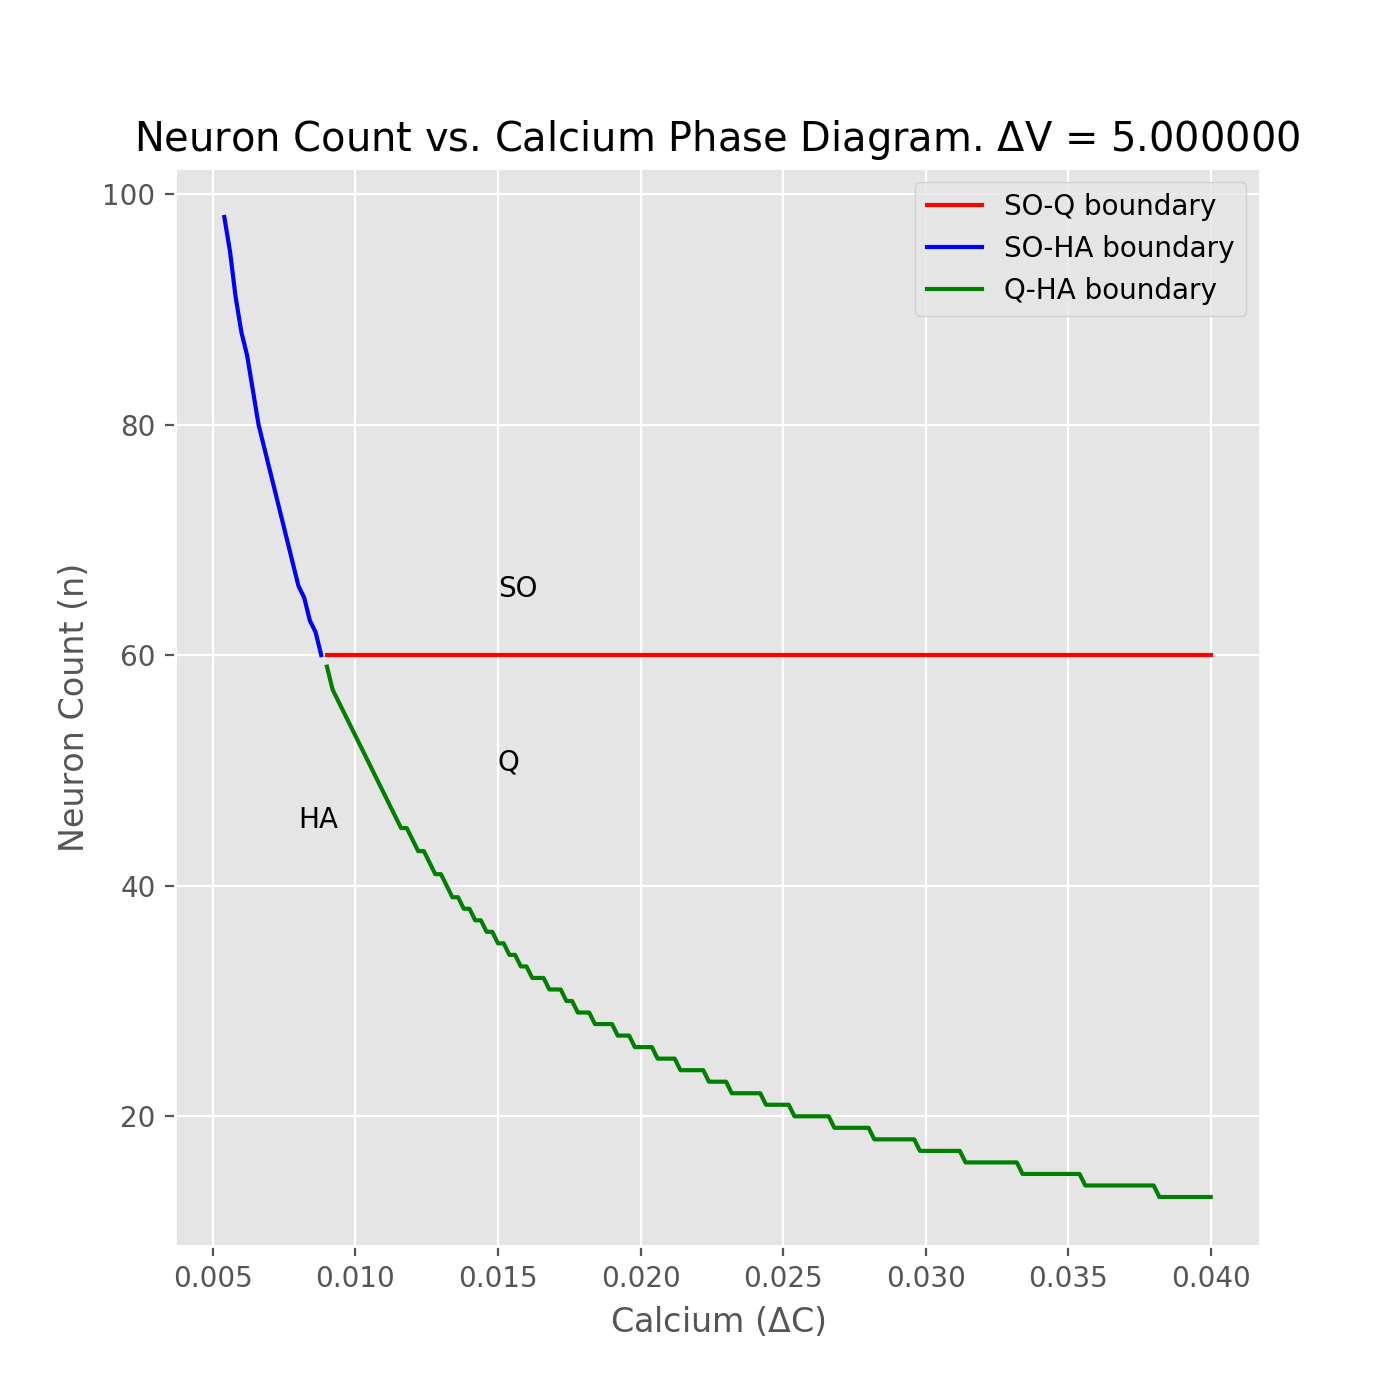
\includegraphics[width=70mm]{step_nC_phase.png}
  \caption{Left: Phase diagram in $\Delta V$. Right: Phase diagram in $\Delta C$.}
  \label{fig:step_function_phase_diagrams}
\end{figure}

\subsection*{Step function without offset from 0}
Network K-cores can be predicted accurately from the step function without an offset from 0. The predicted k-core size was computed using the formula
$$\text{floor}(\frac{V^*}{(r_0 + r_1)\tau _V \Delta V_{min}})$$

\begin{figure}[h!]
  \centering
    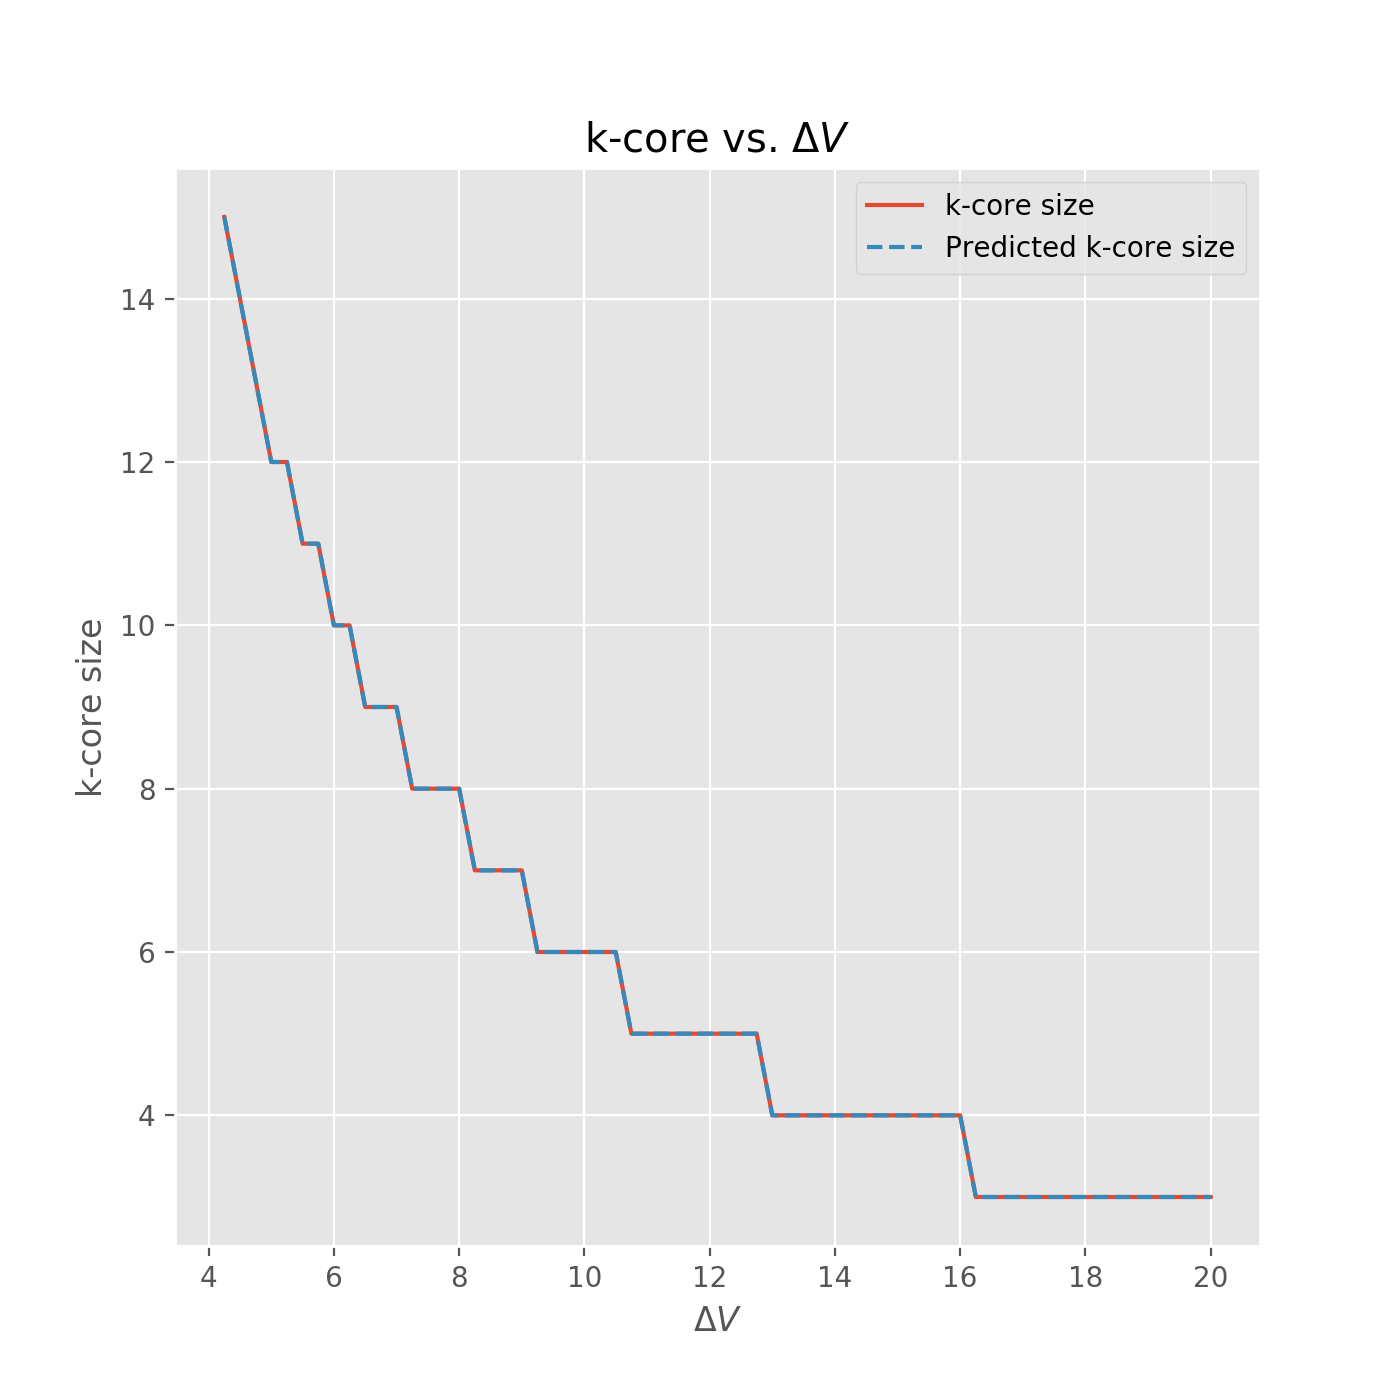
\includegraphics[width=70mm]{kcore_exact_vs_predict.png}
  \caption{Image of k-core size as a function of $\Delta$V.}
  \label{fig:kcore_exact_vs_predict}
\end{figure}

\section*{Sigmoid Function}

\end{document}
